\section{Produit matriciel}

Le produit matriciel est une opération de type BLAS3, qui sont des opérations matrice-matrice. Dans cette partie, nous allons détailler notre implémentation du produit matriciel \texttt{dgemm} ainsi que les optimisations que nous avons effectué, puis nous analyserons les résultats des \emph{benchmarks}.

\subsection{Algorithmes}

Nous avons implémenté la routine \texttt{dgemm} qui effectue un produit matriciel, puis nous avons effectué deux optimisations successives: le produit par blocs et la parallélisation.

Trois types d'algorithmes ont été implémentés : plusieurs séquentiels, un par bloc (reposant sur le précédent) et un parallèle (reposant sur les deux précédents). Ils sont applicables à des matrices de taille quelconque, trois dimensions différentes sont donc prises en compte lorsque l'on cherche à calculer $C \leftarrow \alpha op(A) \times B + \beta C$ :
\begin{itemize}
\item $m$ le nombre de lignes dans $op(A)$  et $C$ ;
\item $n$ le nombre de colonnes dans $B$ et $C$ ;
\item $k$ le nombre de colonnes dans $op(A)$ et de ligne dans $B$.
\end{itemize}


\subsubsection{Problème}

\paragraph{Entrées.} La routine prend comme paramètres:
\begin{itemize}
\item une matrice A de taille $K*M$
\item une matrice B de taille $K*N$
\item une matrice A de taille $M*N$
\item 2 \texttt{double} $\alpha$ et $\beta$
\end{itemize}
La routine CBLAS prend d'autres informations pour modifier l'opération effectuée, mais nous ne les détaillerons pas ici. Celles-ci seront fixées afin d'effectuer l'opération décrite.

Chaque matrice est décrite par les informations suivantes:
\begin{itemize}
\item Un pointeur $A$ vers le premier élément,
\item Un nombre de lignes $M$
\item Un nombre de colonnes $N$
\item Une \textit{leading dimension} \texttt{lda}
\end{itemize}
Une matrice est représentée par colonnes en mémoire, et chaque colonne est espacée de \texttt{lda}.


\paragraph{Sortie.} La routine modifie la matrice $C$ de la manière suivante:
\begin{equation}
C=\beta \cdot C + \alpha \cdot A^T \cdot B 
\end{equation}
Cela se traduit au niveau des coefficients $c_{i,j}$ par la formule suivante:
\begin{equation}
c_{i,j} = \beta c_{i,j} + \alpha \sum\limits_{k=1}^n a_{k,i} \cdot b_{k,j}
\end{equation}


\paragraph{Complexité.} La complexité de cette routine en nombre d'opérations flottantes à double précision est:
\begin{equation}
C(m,n,k)=(2\times k-1)\times m\times n
\end{equation}
Des optimisations sur la complexité sont possibles, comme par exemple grâce à l'algorithme de Strassen, mais ce type d'algorithmes ne s'adapte pas bien au considérations pratiques de ce TDP.


\subsubsection{Algorithme de base}

Cet algorithme est le plus proche de la forme mathématique ci-dessus, il se décompose en trois boucles itérant sur les variables $i,j,k$ de cette formule. Du fait du caractère commutatif de l'addition, l'ordre des calculs n'influe pas sur le résultat. Le point à étudier est alors la différence de performance entre les trois possibilités d'agencement de ces boucles : $ijk$, $jik$, $kij$.

On se doute que les boucles les plus intérieures doivent respecter la cohérence spatiale, c'est à dire parcourir les colonnes des matrices. Ainsi, la boucle sur $k$ (colonnes de $A$ et $B$) devra être la plus intérieure. Dans cette situation, on écrit tous les $c_{i,j}$ les uns après les autres, ce qui permet d'accumuler les résultats dans un registre et de n'écrire qu'une fois $c_{i,j}$ en mémoire.

\subsubsection{Blocs}\label{sec:algo_bloc}

L'algorithme par blocs change l'ordre des calculs en découpant les matrices en blocs, puis en effectuant les produits matriciels des sous-blocs indépendamment avec l'algorithme de base dans sa version $jik$. La taille des blocs est configurable selon les 3 dimensions $i,j,k$.

Le but de cette optimisation est d'augmenter la réutilisation des valeurs stockées dans les caches. En effet, lors de l'exécution de la routine, chaque valeur dans les matrices $A$ est lue $N$ fois. Si les matrices multipliées tiennent en cache, une seule lecture en RAM est nécessaire pour chaque élément. Si la matrice est trop grande, les lignes de cache sont écrasées. On espère donc que le produit par blocs optimise ces accès au cache pour des tailles de blocs suffisamment petites pour rentrer dans les caches.

Après les \emph{benchmarks}, nous avons choisi des blocs de taille $M=512 , N=512 , K=1024$, ce qui correspond expérimentalement aux performances qui nous ont paru être les meilleures

\subsubsection{Parallélisme}

La parallélisation du produit matriciel est possible en découpant la matrice $C$ en autant de blocs que de processeurs, puis en effectuant les sous produits indépendamment sur chaque processeur.

Soit $p$ le nombre de processeurs. La matrice $C$ est découpée en $M_B*N_B$ blocs avec $M_B$ et $N_B$ tels que $M_B*N_B = p$ et $M_B - N_B$ minimal \footnote{$M_B$ est le plus grand diviseur de $p$ inférieur à $\sqrt p$}. Les matrices $A$ et $B$ sont découpées respectivement en blocs de $N_B$ et $M_B$ colonnes.

Chaque coeur calcule indépendamment son sous-produit matriciel avec l'algorithme par blocs.

\subsection{Benchmark}

Nous avons mesuré les performances des différents algorithmes que nous avons implémenté en faisant varier la taille des données en gardant toujours la même distribution en mémoire.

Toutes les matrices utilisées sont carrées de taille $N$ et remplies aléatoirement. L'espace mémoire est réutilisé, les données accédées peuvent donc rester en cache. On utilise 3 espaces de stockage et on garde toujours la même \emph{leading dimension}, ce qui n'est pas forcément bon pour la localité spatiale.

\begin{figure}[!ht]
\centering

\begin{subfigure}[b]{.5\textwidth}
  \centering
  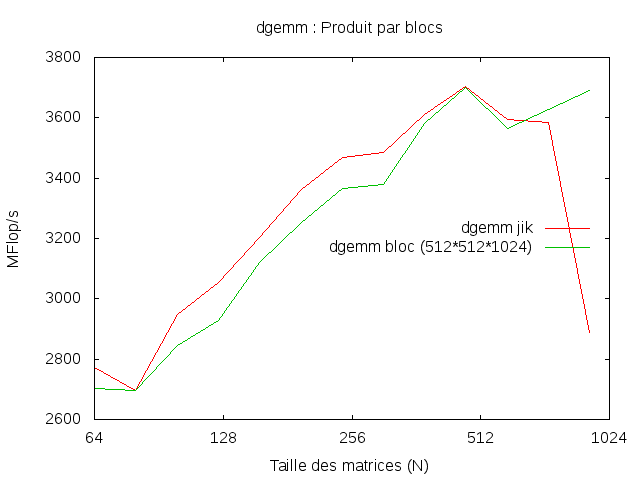
\includegraphics[width=\textwidth]{mat_bloc.png}
  \caption{Optimisation par blocs}
  \label{fig:mat_bloc}
\end{subfigure}%
\begin{subfigure}[b]{.5\textwidth}
  \centering
  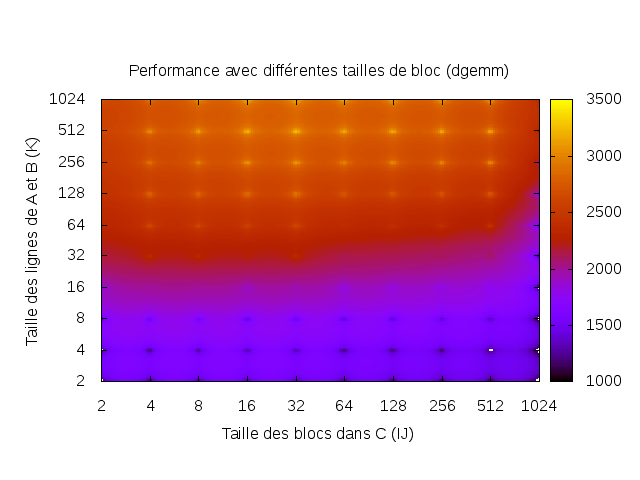
\includegraphics[width=\textwidth]{mat_bloc_size.png}
  \caption{Impact de la taille des blocs}
  \label{fig:mat_bloc_size}
\end{subfigure}

\begin{subfigure}[b]{.5\textwidth}
  \centering
  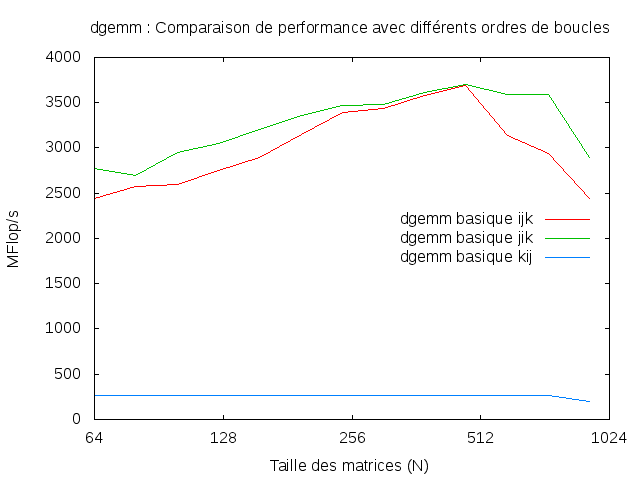
\includegraphics[width=\textwidth]{mat_ijk.png}
  \caption{Impact de l'ordre des boucles}
  \label{fig:mat_ijk}
\end{subfigure}%
\begin{subfigure}[b]{.5\textwidth}
  \centering
  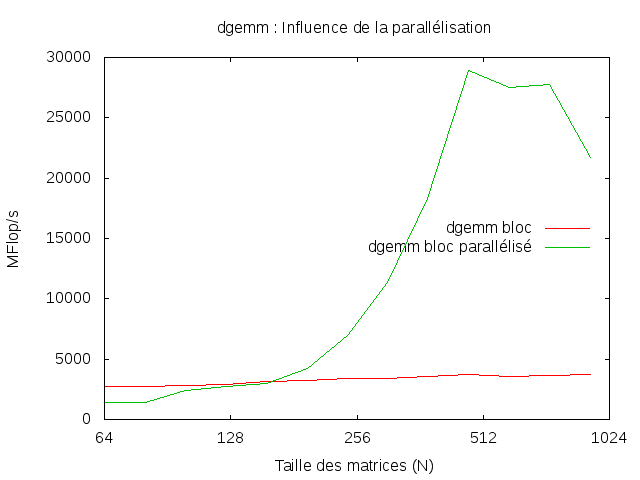
\includegraphics[width=\textwidth]{mat_parallel.png}
  \caption{Résultat de la parallélisation}
  \label{fig:mat_parallel}
\end{subfigure}
\begin{subfigure}[b]{.5\textwidth}
  \centering
  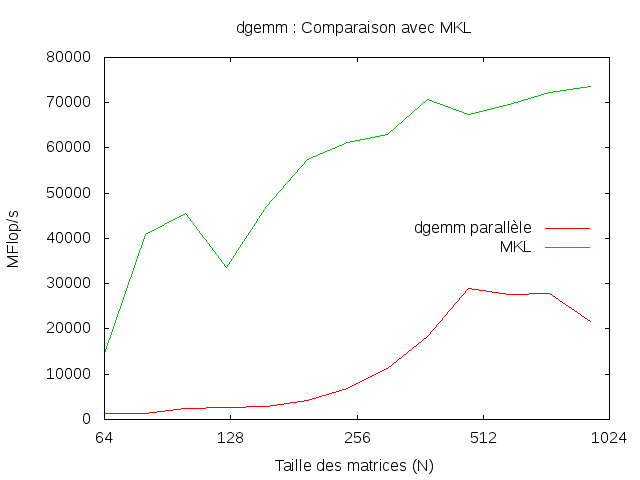
\includegraphics[width=\textwidth]{mat_mkl.png}
  \caption{Comparaison avec MKL}
  \label{fig:mat_mkl}
\end{subfigure}
\caption{Benchmarks pour \texttt{ddot}}
\label{fig:mat}
\end{figure}


\subsubsection{Influence de l'ordre des boucles}

Le graphique \ref{fig:mat_ijk} confirme bien que la boucle su $k$ doit être la plus interne, sinon on perd en performances. Pour l'ordre $kij$ on observe une performance constante d'environ 300 Mflop/s qui correspond probablement à une performance bridée par la bande passante mémoire en écriture dans les $c_{i,j}$.
    
Parcourir les colonnes de $C$ dans la boucle interne ($jik$) donne de légèrement meilleures performances, probablement grâce à la localité spatiale.
    
Les performances augmentent avec les tailles des matrices jusqu'aux environs de $N=512$, au moment ou les matrices remplissent le cache L3 (8Mo).
    
Il est important de noter que ce résultat n'est vrai que lorsque les matrices sont représentées en \texttt{ColMajor} et que $A$ est transposée. On retiendra juste que la boucle la plus interne doit être celle qui préserve la localité spatiale et qui fait toutes les écritures dans un même $c_{i,j}$ à la suite.


\subsubsection{Influence des blocs}

Le graphique \ref{fig:mat_bloc} montre dans quelle mesure le produit par blocs optimise les performances. Les performances sont légèrement moins bonnes jusqu'au moment où le produit $jik$ atteint son maximum de performances. Après ce cap, les performances du produit $jik$ régressent alors que celles du produit bloc restent constantes. Cela est probablement dû au phénomène décrit en \ref{sec:algo_bloc}: le produit bloc réutilise mieux les valeurs en cache.
    
Nous pouvons imaginer que la taille des blocs optimale est atteinte lorsque les blocs remplissent le cache; c'est pourquoi nous avons choisi de découper $C$ en blocs de taille $512*512$ et de prendre des lignes de taille $1024$ afin de garder de la cohérence spatiale.
    
\paragraph{Influence de la taille des blocs}
    
Nous avons aussi voulu montrer quel était l'influence de la taille des blocs sur les performances pour des matrices de taille $1024*1024$. La figure \ref{fig:mat_bloc_size} donne les performances en fonction de deux paramètre: $ij$ la taille des carrés qui composent $C$, et $k$ la taille des lignes dans les matrices $A$ et $B$. 
    
Des points brillants représentent des pics de performances proche des puissances de 2, probablement liés à l'alignement mémoire. On observe que pour avoir de bonnes performances, il faut que les lignes (dimension $K$) soient suffisamment grandes ; sinon les performances sont désastreuses, à l'image de l'algorithme $kij$. Dans ces plages de taille, l'influence de $ij$ n'est pas bien mise en avant, mais le temps de calcul avec des matrices plus grandes devenait trop long. Il semble tout de même que les performances diminuent lorsque $ij$ devient trop grand, et que les points semblent plus brillants lorsque $ij$ est de l'ordre de 32. 
    
L'idéal est donc de prendre des grandes lignes, et de subdiviser $C$ en des matrices plus petites, à priori on a de meilleures performances si les blocs tiennent dans le cache.
    
    
\subsubsection{Influence du parallélisme}

Pour les données sur le parallélisme, le nombre de \emph{threads} créé est de 8.

La figure \ref{fig:mat_parallel} montre le résultat de la parallélisation. Pour des petites tailles, la parallélisation est plus coûteuse que l'algorithme séquentiel, probablement à cause de la mise en place des \emph{threads}. A partir d'une taille de l'ordre de 128 on observe que les performances croissent linéairement en fonction de la taille jusqu'à une taille de 512. L'algorithme est alors à peu près 8 fois plus rapide, ce qui est cohérent avec le nombre de coeurs de la machine.
    
Dans la figure \ref{fig:mat_mkl}, MKL fait 4 fois mieux que notre routine et plafonne à un peu moins de 80 GFlop/s, ce qui semble représenter la puissance crête d'un processeur X5550. Nous nous demandons donc si les 8 \emph{threads} sont distribués sur un seul processeur \emph{hyperthreadé} parmi les 2 processeurs d'un noeud de calcul. Mais nous n'avons pas pu confirmer cette hypothèse.
    
    